 %% stack-example.tex
  %% Copyright 2010 Matthieu Moy <Matthieu.Moy@imag.fr>
  %
  % This work may be distributed and/or modified under the
  % conditions of the LaTeX Project Public License, either version 1.3
  % of this license or (at your option) any later version.
  % The latest version of this license is in
  %   http://www.latex-project.org/lppl.txt
  % and version 1.3 or later is part of all distributions of LaTeX
  % version 2005/12/01 or later.
  %
  % This work has the LPPL maintenance status `maintained'.
  %
  % The Current Maintainer of this work is M. Matthieu Moy.
  %
  % This work consists of the files drawstack.sty and the example file
  % stack-example.tex.

\documentclass{article}

\usepackage{drawstack}

% Use this instead if you don't want colors.
% \usepackage[nocolor]{drawstack}

\title{{\tt drawstack.sty}: Draw execution stack easily in LaTeX}
\author{Matthieu Moy}

\begin{document}
\maketitle

{\tt drawstack} is a LaTeX package to easily draw execution stack
(typically to illustrate assembly language notions), written on top of
TikZ. This file serves as an example of usage of {\tt drawstack}, and
serves as documentation for this package. Read the source code and
comments to see how to use it.

\section{Minimalistic example}

% The main feature of the package is to define an environment
% drawstack.
\begin{drawstack}
  % Within the environment, draw stack elements with \cell{...}
  \cell{First cell}
  \cell{Second cell}
\end{drawstack}

\section{Grouping cells into stack frames}

\begin{drawstack}
  \startframe
  \cell{First cell}
  \cell{Second cell}
  \finishframe{Some stack frame}
  \cell{Not interesting}
  \startframe
  \cell{Next stack frame}
  \cell{Next stack frame}
  \finishframe{Another stack frame}
\end{drawstack}

\section{Stack and Base pointers}

\begin{drawstack}
  \startframe
  % \cellcom writes something on the right-hand side of a cell.
  \cell{loc2} \cellcom{-8(\%ebp)}
  \cell{loc1} \cellcom{-4(\%ebp)}
  % \esp and \ebp are stack pointer and base pointer in Pentium.
  % These macros are simple shortcuts for \cellptr{...}
  \cell{Sauvegarde \%ebp} \esp \ebp
  \cell{@ retour} \cellcom{4(\%ebp)}
  \finishframe{fonction\\ {\tt f}}
  \startframe
  \cell{} \cellcom{8(\%ebp)}
  \cell{}
  \finishframe{fonction\\ {\tt main}}
\end{drawstack}

\section{Padding}

\begin{drawstack}
  \cell{above padding}
  \padding{3}{nothing here}
  \cell{below padding}
\end{drawstack}

\section{Below/Above stack pointer}

\begin{drawstack}
  \cell{Top}
  \cell{Below top}
  % \bcell is just like \cell, but in a different color.
  \bcell{Above bottom} \cellptr{Stack pointer here}
  \bcell{Bottom}
\end{drawstack}

\section{Highlighting some cell}

\begin{drawstack}
  \cell{Uninteresting cell}
  \cell{Interesting cell} \cellround{Yes, this one!}
\end{drawstack}

\section{Structures without a stack structure}

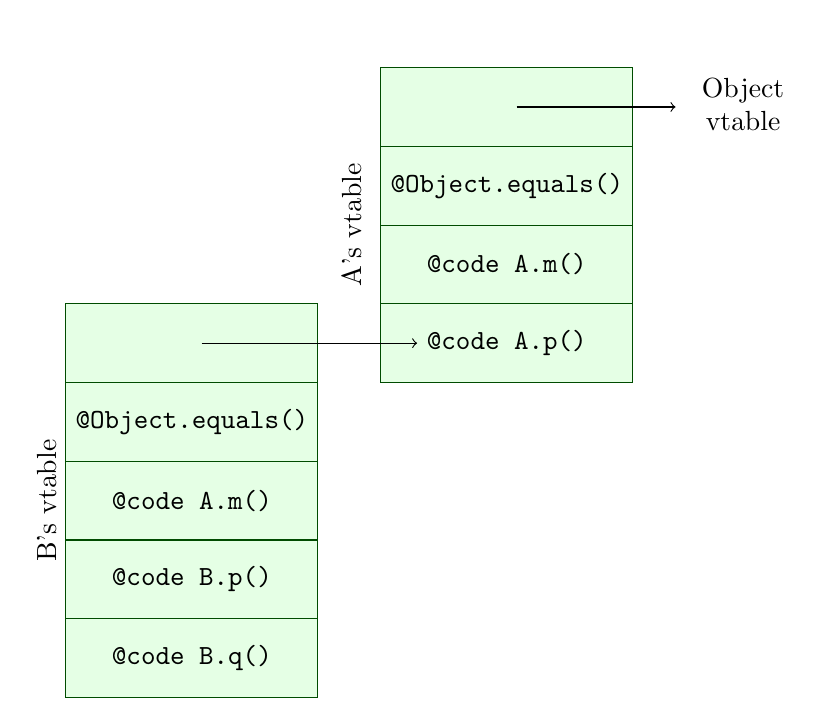
\begin{tikzpicture}
  \draw (3, -1) node (Otm) {
    \begin{tabular}{c}
      Object\\vtable
    \end{tabular}
  };

  \drawstruct{(0,0)}
  \structcell[freecell]{~} \coordinate (Atm) at (currentcell.east);
  \structcell[freecell]{\texttt{@Object.equals()}}
  \structcell[freecell]{\texttt{@code A.m()}}
  \structcell[freecell]{\texttt{@code A.p()}} \coordinate (A) at (currentcell.west);
  \structname{
    \begin{tabular}{c}
      A's vtable
    \end{tabular}
  }

  \drawstruct{(-4,-3)}
  \structcell[freecell]{} \coordinate (Btm) at (currentcell.east);
  \structcell[freecell]{\texttt{@Object.equals()}}
  \structcell[freecell]{\texttt{@code A.m()}}
  \structcell[freecell]{\texttt{@code B.p()}}
  \structcell[freecell]{\texttt{@code B.q()}}
  \structname{B's vtable}

  \draw[->] (Btm) -- (A);
  \draw[->] (Atm) -- (Otm);
\end{tikzpicture}

\section{Structures and stack together}

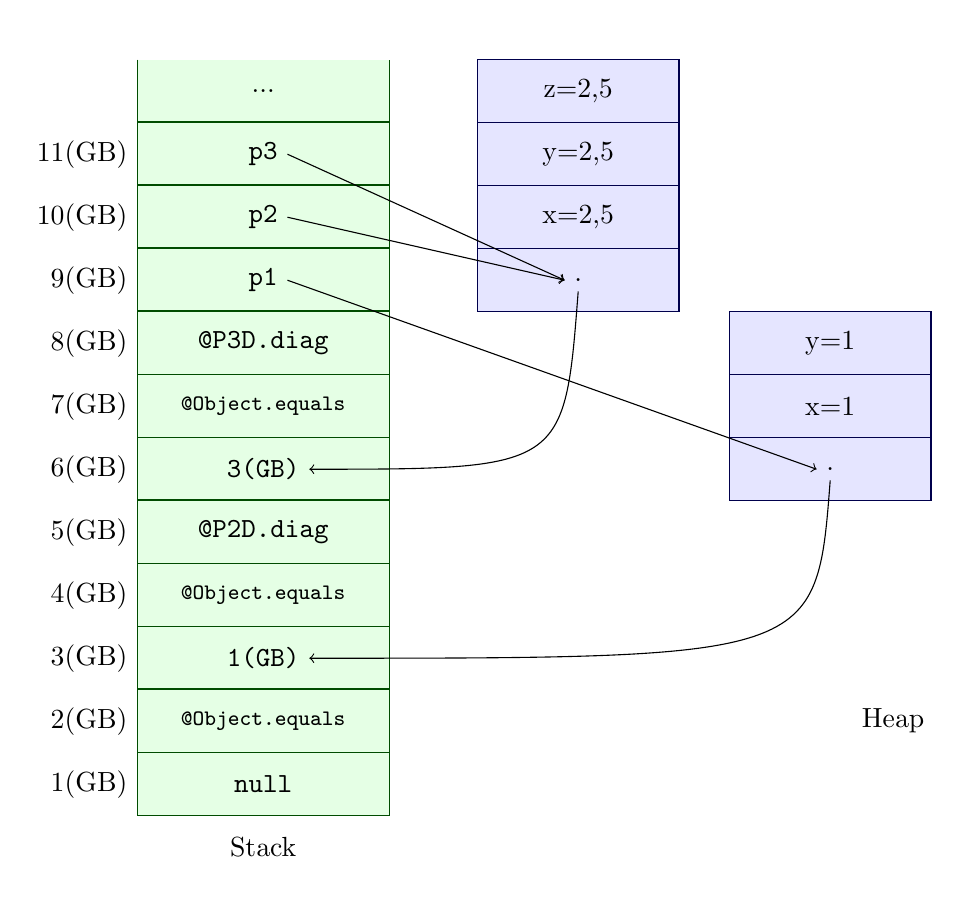
\begin{tikzpicture}[scale=.8]

  \stacktop{}
  \separator
  \cell{\texttt{p3}}        \cellcomL{11(GB)} \coordinate (p3) at (currentcell.east);
  \separator
  \cell{\texttt{p2}}        \cellcomL{10(GB)} \coordinate (p2) at (currentcell.east);
  \separator
  \cell{\texttt{p1}}        \cellcomL{ 9(GB)} \coordinate (p1) at (currentcell.east);
  \separator
  \cell{\texttt{@P3D.diag}} \cellcomL{ 8(GB)}
  \cell{\texttt{\footnotesize @Object.equals}} \cellcomL{ 7(GB)}
  \cell{\texttt{3(GB)}}     \cellcomL{ 6(GB)} \coordinate (T1) at (currentcell.east);
  \separator
  \cell{\texttt{@P2D.diag}} \cellcomL{ 5(GB)}
  \cell{\texttt{\footnotesize @Object.equals}} \cellcomL{ 4(GB)}
  \cell{\texttt{1(GB)}}     \cellcomL{ 3(GB)} \coordinate (T2) at (currentcell.east);
  \separator
  \cell{\texttt{\footnotesize @Object.equals}} \cellcomL{ 2(GB)}
  \cell{\texttt{null}}      \cellcomL{ 1(GB)}
  \cell[draw=none]{Stack}


  \drawstruct{(5,1)})
  \structcell{z=2,5}
  \structcell{y=2,5}
  \structcell{x=2,5}
  \structcell{.} \coordinate (O1) at (currentcell.west);
  \coordinate (O1l) at (currentcell.south);

  \drawstruct{(9,-3)}
  \structcell{y=1}
  \structcell{x=1}
  \structcell{.} \coordinate (O2) at (currentcell.west);
  \coordinate (O2l) at (currentcell.south);

  \draw[->] (p3) -- (O1);
  \draw[->] (p2) -- (O1);
  \draw[->] (p1) -- (O2);

  \draw[->] (O1l) .. controls (O1 |- T1) .. (T1);
  \draw[->] (O2l) .. controls (O2 |- T2) .. (T2);

  \draw (10,-10) node{Heap};

\end{tikzpicture}



\section{Using tikzpicture instead of drawstack}

% The environment drawstack is basically a syntactic sugar for
%
% \begin{tikzpicture}[#1]
% \stacktop{}
% ...
% \stackbottom
% \end{tikzpicture}
%
% You can use the above syntax for more flexibility.

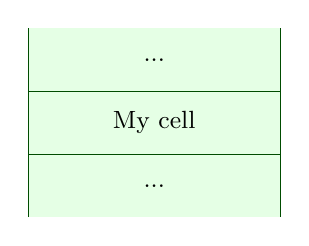
\begin{tikzpicture}[scale=0.8]
  \small
  \stacktop{}
  \cell{My cell}
  \stackbottom{}
\end{tikzpicture}

\section{Changing style}

{% tikzstyle will be local to this {...}
\tikzstyle{freecell}=[fill=blue!10,draw=blue!30!black]
\tikzstyle{occupiedcell}=[fill=blue!10!orange!10,draw=blue!30!black]
\tikzstyle{padding}=[fill=yellow!20,draw=blue!30!black]
\tikzstyle{highlight}=[draw=orange!50!black,text=orange!50!black]

\begin{drawstack}
  \cell{Uninteresting cell}
  \cell{Interesting cell} \cellround{Yes, this one!}
  \bcell{bcell}
  \padding{2}{Padding}
\end{drawstack}
}

\section{Example: Computing Factorial}

\begin{drawstack}[scale=0.8]
  \startframe
  \cell{N = 1}
  \cell{...}
  \finishframe{fact(1)}
  \startframe
  \cell{N = 2}
  \cell{...}
  \finishframe{fact(2)}
  \cell{$\vdots$}
  \startframe
  \cell{N = 5}
  \cell{...}
  \finishframe{fact(5)}
\end{drawstack}

\end{document}

%%% Local Variables:
%%% mode: latex
%%% TeX-master: t
%%% End:
